%\documentclass[twocolumn,amsmath,amssymb]{report}
\documentclass[twocolumn,amsmath,amssymb]{snp}
\pagestyle{empty}
\usepackage{graphicx}% Include figure files
\usepackage{dcolumn}% Align table columns on decimal point
\usepackage{bm}% bold math
\topmargin 1.5 cm
\textwidth14.5cm
\textheight20cm
\oddsidemargin0.7cm
\columnsep0.2in
\begin{document}

%\title{{\Large Using Machine learning to segregate cosmic muons from background gammas}}% Force line breaks with \\
\title{{\Large Using Machine learning to segregate cosmic muons from background events}}

\author{\large R. Sehgal$^1$}
\email{rsehgal@barc.gov.in}
\author{\large S. P. Behera$^1$}
\author{\large K. Kumar$^1$}
\author{\large P. K. Netrakanti$^1$}
\author{\large D. K. Mishra$^{1,2}$}
\author{\large V. Jha$^{1,2}$}

% \altaffiliation[Also at ]{Physics Department, XYZ University.}%Lines break automatically or can be forced with \\
\affiliation{$^1$Nuclear Physics Division, Bhabha Atomic Research Centre, Mumbai - 400085, INDIA}
\affiliation{$^2$Homi Bhabha National Institute, Anushaktinagar, Mumbai - 400094, INDIA}
%\affiliation{$^3$Inter University Accelerator Centre, Aruna Asaf Ali Marg, New Delhi - 110067, INDIA}
%\affiliation{$^4$Physics Department, XYZ University}
\maketitle


\section*{Introduction}
Cosmic muons are high-energy charged particles originating from cosmic rays in the upper atmosphere and reaches the Earth surface. These cosmic muons has the mean energy of $\sim$ 3-4 GeV, which make them a particularly useful probe for applications like Muon Tomography, and can also be used as a probe to calibrate particle detectors. In addition to cosmic muons, several order of magnitude more cosmic background is also available in our environment. Hence, these cosmic muons need to be segregated from background events depending upon the application specific muon trigger condition. In the current work we will present a Machine Learning based approach to segregate these cosmic muon from background gamma where the muon trigger is the coincidence between the two layers of plastic scintillator detectors separated by $\sim$1m.

\section*{Detector Setup} %\label{detector}
The detector setup consist of plastic scintillator matrix of ISMRAN detector \cite{rdey}. It consist of 90 scintillator bars arranged in a matrix of 9 $\times$ 10. Each plastic scintillator bar (10 cm $\times$ 10 cm $\times$ 100 cm) is coupled to the Photo Multiplier Tube (PMT) at both ends, which are used to get the timing and the integrated charge. The geometric mean of these integrated charges correspond to the energy deposited in the scintillator by the incident radiation, and is key to segregate the cosmic muon from background events in conventional techniques.
%, as it is seen from the GEANT4 \cite{geant} simulation that cosmic muons deposit $\sim$2MeV/cm for the material used in the scintillator bar which is much more than the energy deposited by background $\gamma$ rays.
%The energy based segregation procedure requires the energy calibration to be applied on the integrated charge, so that it integrated charge represents the energy deposited.

%\section*{Conventional energy calibration procedure}
\section*{Conventional energy deposition based cosmic muon segregation}
Conventionally cosmic muons are segregated from the background based on the energy deposition threshold \cite{mypaper}, which involves the energy calibration of these detectors. Fig. \ref{calib} shows the plot of energy deposited by cosmic particles after the application of energy calibration. The energy deposited by cosmic muons peaked at $\sim$20MeV, which is also verified using GEANT4 \cite{geant} simulation. Hence, an appropriate energy threshold $\sim$8-10 MeV may be chosen to segregate the cosmic muons hits from the background. To further make sure that the selected events are muon events, a trigger may be generated by taking the coincidence of two layers of scintillator separated by a distance of $\sim$1m. Hence an event will be considered as muon event only if crosses the energy deposition threshold and forms a muon trigger.
%The energy calibration of these detectors are conventionally done using different radioactive sources of known energies to get a parameterization to map the integrated charge to energy. The parameterization will then be applied on the experimental data to get the energy deposited by incident radiation. Fig. \ref{calib} shows the plot of energy deposited by cosmic particles after the application of energy calibration. From here one can see that the energy deposited by cosmic muons peaked at $\sim$20MeV, which is also verified using GEANT4 simulation \cite{mypaper}. Hence, an appropriate energy threshold $\sim$10 MeV may be chosen to segregate the cosmic muons hits from the background. To further make sure that the selected events are muon events, a trigger may be generated by taking the coincidence of two layers of scintillator separated by a distance of $\sim$1m. Hence an event will be considered as muon event only if crosses the energy deposition threshold and forms a muon trigger.
\begin{figure}
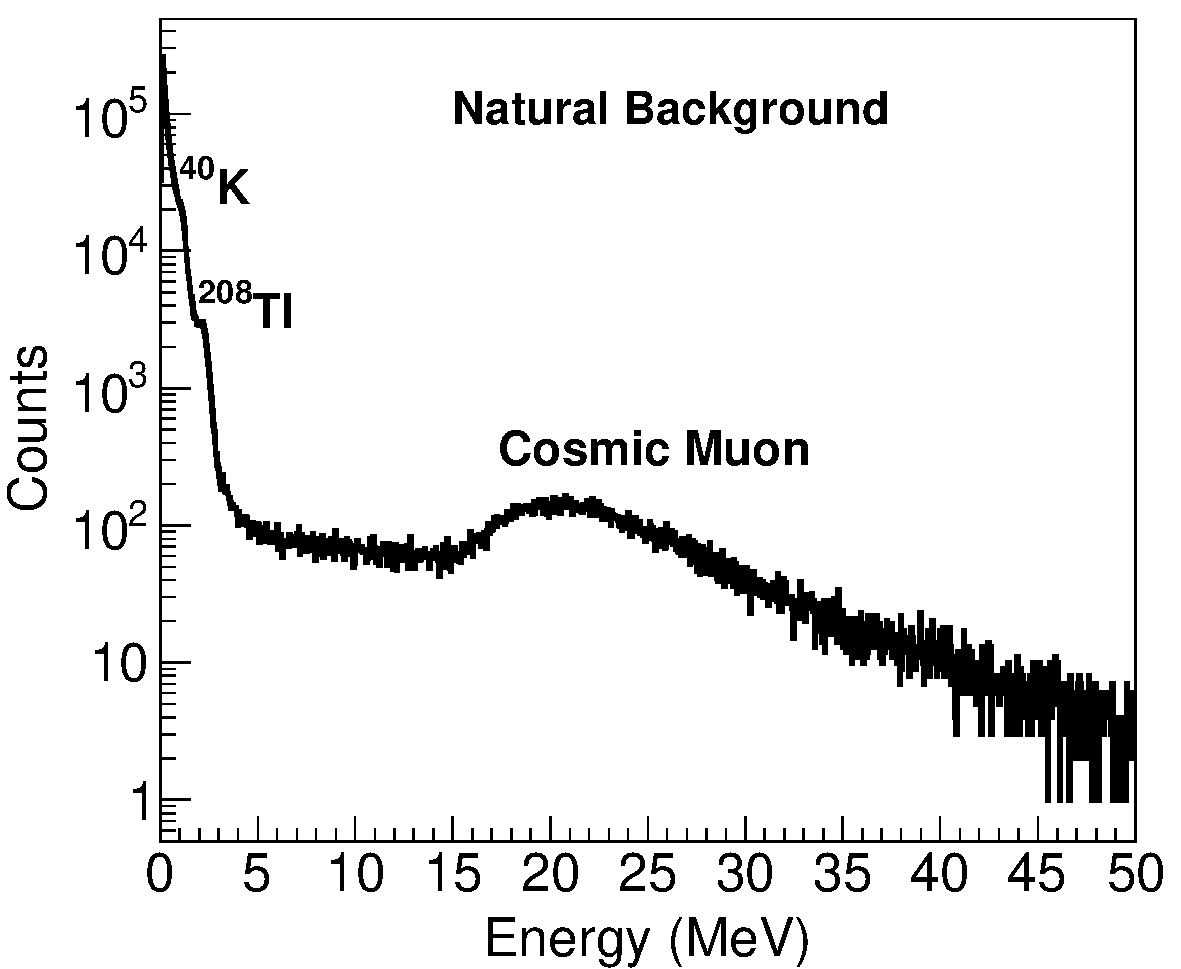
\includegraphics[width=66mm]{calibrated.pdf}% Here is how to import jpg/ png/ pdf figure if you are using pdflatex command to compile
\caption{\label{calib} Spectrum of energy calibrated background $\gamma$ and cosmic muons}
\end{figure}

\section*{Machine learning based cosmic muon segregation}
The conventional approach needs energy calibration procedure followed by muon trigger generation check for individual event to be declared as muon event. This makes the job computation intensive as background events are orders of magnitude more than muon events. Machine learning can help solving the problem where the muon segregation problem can be seen as the binary classfication problem, which can be solved by building a classfication model. The built model can later be used to quickly discriminate background and muon events without applying any energy calibration or trigger generation. Calibrated data and trigger is required only in the initial phase to label the individual events as muon event or background event, which is required for training the classfication model.
%Hence the problem of cosmic muon segregation can be mapped to binary classfication problem in machine learning, as we just want to classify events as muon events or background $\gamma$ events.

\section*{Data Sets}
As mentioned above%in section \ref{detector}
, the data from experiment consist of timing and integrated charge.
%, where the geometric mean of the integrated charge is proportional to the energy deposited.
In the present work, both the parameters are used as the features for the segregation of cosmic muon. For the learning phase of the model, the timing and integrated charge obtained from both the PMTs are used as the input features. The minimum energy deposition threshold is kept at 3 MeV, so that the muons which are just grazed through the detector should also get recorded. The event is labelled as muon event if the energy deposited is more than the threshold value and a coincidence is found between the
%two layers of scintillators which are separated by $\sim$1m ,
top and the bottom layer, which are separated by $\sim$1m, otherwise it is labelled as background event. 
%The labelled data set is used to train and test the classfication model and the results are shown below.
\section*{Results}
 After building the labelled dataset, a regression based classfication model is trained using 3 $\times$ $10^{5}$ events of labelled data. To evaluate the performance of the classification model, another labelled dataset of 3 $\times$ $10^{5}$ events is used, and muon classification performance of the model is found to be $\sim$95\%. Later on the same model is applied on the input features of raw data  %i.e. integrated charge and the timing recorded by both the PMTs and
  without applying any energy calibration. Once the classfication is over, the energy calibration is applied only on those events which are classified as muons, and the data is compared with the calibrated data of the complete spectrum, as show in Fig. \ref{classfication}. Here one can see in the red plot, that there are very few low energy background events which are classified as muons, but from $\sim$10-11 MeV onwards we are able to correctly classify them as muons, which we had previously verified by GEANT4 simulations.

\begin{figure}
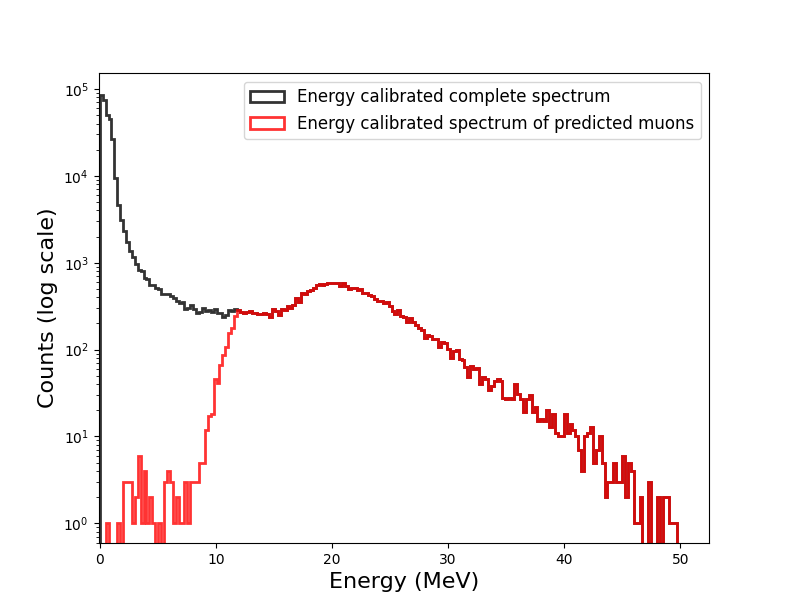
\includegraphics[width=66mm]{prediction2.png}% Here is how to import jpg/ png/ pdf figure if you are using pdflatex command to compile
\caption{\label{classfication} Muons segregation using Machine learning classification algorithm}
\end{figure}
\section*{Conclusion}
By harnessing the power of advanced machine learning classification algorithms, a successful segregation between cosmic muons and background events is obtained based on their distinct energy deposition and timing patterns. This has yielded the promising results with significant implications for applications like Muon Tomography. \\

%The application of machine learning techniques to segregate cosmic muons from background $\gamma$ rays has yielded promising results with significant implications for applications like Muon Tomography. By harnessing the power of advanced classification algorithms, a successfulsegregation between cosmic muons and background $gamma$-rays is obtained based on their distinct energy deposition patterns. 

%Moreover, the successful segregation  through machine learning not only refines our understanding of the underlying physical phenomena but also paves the way for more precise measurements, deeper insights into particle interactions, and more efficient utilization of experimental resources in the quest for unraveling the mysteries of the cosmos.


% These machine learning models leverage sophisticated feature extraction and pattern recognition, allowing for accurate identification even in complex and noisy environments. The outcomes of these efforts include enhanced data purity in experiments sensitive to rare processes, improved calibration procedures, and reduced systematic uncertainties.

\iffalse
\begin{table}[h]
\caption{\label{tab:table1}This is a table which fits
properly in a column. Note that several entries share the same
footnote. Inspect the \LaTeX\ input for this table to see
exactly how it is done.}
\begin{tabular}{|c|c|c|c|c|c|c|}
\hline 
&$r_c$ (\AA)& $r_0$ (\AA)& $\kappa r_0$&
 &$r_c$ (\AA) &$r_0$ (\AA)\\ \hline
Cu& 0.800 & 14.10 & 2.550 &Sn\footnotemark[1]
& 0.680 & 1.870 \\
Ag& 0.990 & 15.90 & 2.710 &Pb\footnotemark[2]
& 0.450 & 1.930  \\
Au& 1.150 & 15.90 & 2.710 &Ca\footnotemark[3]
& 0.750 & 2.120 \\
Mg& 0.490 & 17.60 & 3.200 &Sr\footnotemark[4]
& 0.900 & 2.370 \\
Zn& 0.300 & 15.20 & 2.970 &Li\footnotemark[2]
& 0.380 & 1.730 \\
\hline
\end{tabular}
\end{table}
\fi

%\section*{Acknowledgments}
% We thank you for your co-operation in using this template  for production of camera ready manuscript.
%\acknowledgments

%\end{acknowledgments}

%\ \\
%\noindent
\begin{thebibliography}{50}
\bibitem{rdey} R. Dey et al., \emph{NIMA} {\bf 1042}, {\bf 2022}
\bibitem{mypaper} R. Sehgal et al., \emph{JINST} {\bf 17} P02036,  September {\bf 2022}
\bibitem{geant} S. Agostinelli et al., \emph{GEANT4, NIM-A} {\bf 506}, 250, {\bf 2003}

\end{thebibliography}

\end{document}
%
% ****** End of file snpcontrisamp.tex ******
